% Options for packages loaded elsewhere
\PassOptionsToPackage{unicode}{hyperref}
\PassOptionsToPackage{hyphens}{url}
%
\documentclass[
]{article}
\usepackage{lmodern}
\usepackage{amssymb,amsmath}
\usepackage{ifxetex,ifluatex}
\ifnum 0\ifxetex 1\fi\ifluatex 1\fi=0 % if pdftex
  \usepackage[T1]{fontenc}
  \usepackage[utf8]{inputenc}
  \usepackage{textcomp} % provide euro and other symbols
\else % if luatex or xetex
  \usepackage{unicode-math}
  \defaultfontfeatures{Scale=MatchLowercase}
  \defaultfontfeatures[\rmfamily]{Ligatures=TeX,Scale=1}
\fi
% Use upquote if available, for straight quotes in verbatim environments
\IfFileExists{upquote.sty}{\usepackage{upquote}}{}
\IfFileExists{microtype.sty}{% use microtype if available
  \usepackage[]{microtype}
  \UseMicrotypeSet[protrusion]{basicmath} % disable protrusion for tt fonts
}{}
\makeatletter
\@ifundefined{KOMAClassName}{% if non-KOMA class
  \IfFileExists{parskip.sty}{%
    \usepackage{parskip}
  }{% else
    \setlength{\parindent}{0pt}
    \setlength{\parskip}{6pt plus 2pt minus 1pt}}
}{% if KOMA class
  \KOMAoptions{parskip=half}}
\makeatother
\usepackage{xcolor}
\IfFileExists{xurl.sty}{\usepackage{xurl}}{} % add URL line breaks if available
\IfFileExists{bookmark.sty}{\usepackage{bookmark}}{\usepackage{hyperref}}
\hypersetup{
  pdftitle={ETC3250/5250 Assignment 1},
  hidelinks,
  pdfcreator={LaTeX via pandoc}}
\urlstyle{same} % disable monospaced font for URLs
\usepackage[margin=1in]{geometry}
\usepackage{color}
\usepackage{fancyvrb}
\newcommand{\VerbBar}{|}
\newcommand{\VERB}{\Verb[commandchars=\\\{\}]}
\DefineVerbatimEnvironment{Highlighting}{Verbatim}{commandchars=\\\{\}}
% Add ',fontsize=\small' for more characters per line
\usepackage{framed}
\definecolor{shadecolor}{RGB}{248,248,248}
\newenvironment{Shaded}{\begin{snugshade}}{\end{snugshade}}
\newcommand{\AlertTok}[1]{\textcolor[rgb]{0.94,0.16,0.16}{#1}}
\newcommand{\AnnotationTok}[1]{\textcolor[rgb]{0.56,0.35,0.01}{\textbf{\textit{#1}}}}
\newcommand{\AttributeTok}[1]{\textcolor[rgb]{0.77,0.63,0.00}{#1}}
\newcommand{\BaseNTok}[1]{\textcolor[rgb]{0.00,0.00,0.81}{#1}}
\newcommand{\BuiltInTok}[1]{#1}
\newcommand{\CharTok}[1]{\textcolor[rgb]{0.31,0.60,0.02}{#1}}
\newcommand{\CommentTok}[1]{\textcolor[rgb]{0.56,0.35,0.01}{\textit{#1}}}
\newcommand{\CommentVarTok}[1]{\textcolor[rgb]{0.56,0.35,0.01}{\textbf{\textit{#1}}}}
\newcommand{\ConstantTok}[1]{\textcolor[rgb]{0.00,0.00,0.00}{#1}}
\newcommand{\ControlFlowTok}[1]{\textcolor[rgb]{0.13,0.29,0.53}{\textbf{#1}}}
\newcommand{\DataTypeTok}[1]{\textcolor[rgb]{0.13,0.29,0.53}{#1}}
\newcommand{\DecValTok}[1]{\textcolor[rgb]{0.00,0.00,0.81}{#1}}
\newcommand{\DocumentationTok}[1]{\textcolor[rgb]{0.56,0.35,0.01}{\textbf{\textit{#1}}}}
\newcommand{\ErrorTok}[1]{\textcolor[rgb]{0.64,0.00,0.00}{\textbf{#1}}}
\newcommand{\ExtensionTok}[1]{#1}
\newcommand{\FloatTok}[1]{\textcolor[rgb]{0.00,0.00,0.81}{#1}}
\newcommand{\FunctionTok}[1]{\textcolor[rgb]{0.00,0.00,0.00}{#1}}
\newcommand{\ImportTok}[1]{#1}
\newcommand{\InformationTok}[1]{\textcolor[rgb]{0.56,0.35,0.01}{\textbf{\textit{#1}}}}
\newcommand{\KeywordTok}[1]{\textcolor[rgb]{0.13,0.29,0.53}{\textbf{#1}}}
\newcommand{\NormalTok}[1]{#1}
\newcommand{\OperatorTok}[1]{\textcolor[rgb]{0.81,0.36,0.00}{\textbf{#1}}}
\newcommand{\OtherTok}[1]{\textcolor[rgb]{0.56,0.35,0.01}{#1}}
\newcommand{\PreprocessorTok}[1]{\textcolor[rgb]{0.56,0.35,0.01}{\textit{#1}}}
\newcommand{\RegionMarkerTok}[1]{#1}
\newcommand{\SpecialCharTok}[1]{\textcolor[rgb]{0.00,0.00,0.00}{#1}}
\newcommand{\SpecialStringTok}[1]{\textcolor[rgb]{0.31,0.60,0.02}{#1}}
\newcommand{\StringTok}[1]{\textcolor[rgb]{0.31,0.60,0.02}{#1}}
\newcommand{\VariableTok}[1]{\textcolor[rgb]{0.00,0.00,0.00}{#1}}
\newcommand{\VerbatimStringTok}[1]{\textcolor[rgb]{0.31,0.60,0.02}{#1}}
\newcommand{\WarningTok}[1]{\textcolor[rgb]{0.56,0.35,0.01}{\textbf{\textit{#1}}}}
\usepackage{graphicx,grffile}
\makeatletter
\def\maxwidth{\ifdim\Gin@nat@width>\linewidth\linewidth\else\Gin@nat@width\fi}
\def\maxheight{\ifdim\Gin@nat@height>\textheight\textheight\else\Gin@nat@height\fi}
\makeatother
% Scale images if necessary, so that they will not overflow the page
% margins by default, and it is still possible to overwrite the defaults
% using explicit options in \includegraphics[width, height, ...]{}
\setkeys{Gin}{width=\maxwidth,height=\maxheight,keepaspectratio}
% Set default figure placement to htbp
\makeatletter
\def\fps@figure{htbp}
\makeatother
\setlength{\emergencystretch}{3em} % prevent overfull lines
\providecommand{\tightlist}{%
  \setlength{\itemsep}{0pt}\setlength{\parskip}{0pt}}
\setcounter{secnumdepth}{-\maxdimen} % remove section numbering

\title{ETC3250/5250 Assignment 1}
\author{}
\date{\vspace{-2.5em}DUE: Friday Mar 27, 5pm}

\begin{document}
\maketitle

\hypertarget{instructions}{%
\subsection{Instructions}\label{instructions}}

\begin{itemize}
\tightlist
\item
  You need to turn into moodle, the two files, your \texttt{Rmd} and
  \texttt{html} files.
\item
  \textbf{List your team members as authors} on the report. For each of
  the four assignments, one team member needs to be nominated as the
  leader, and is responsible for coordinating the efforts of other team
  members, and submitting the assignment.
\item
  The expected mode of working is that \textbf{you individually complete
  the assignment}, and then compare your answers and explanations with
  your team mates. Each student will have the opportunity to report on
  other team member's efforts on the assignment, and also report on
  their own lack of contribution. If a member does not substantially
  contribute to the team submission they may get a reduced mark. If a
  team member fails to report their lack of contribution they will
  receive a zero mark.
\item
  R code should be hidden in the final report, unless it is specifically
  requested.
\item
  Original work is expected. Any material used from external sources
  needs to be acknowledged and cited appropriately.
\item
  To make it a little easier for you, a skeleton of R code is provided
  in the \texttt{Rmd} file. Where you see \texttt{???} means that
  something is missing and you will need to fill it in with the
  appropriate function, argument or operator. You will also need to
  rearrange the code as necessary to do the calculations needed.
\end{itemize}

\hypertarget{marks}{%
\subsection{Marks}\label{marks}}

\begin{itemize}
\tightlist
\item
  Total mark will be out or 25
\item
  5 points will be reserved for readability, and appropriate citing of
  external sources
\item
  5 points will be reserved for reproducibility, that the report can be
  re-generated from the submitted Rmarkdown.
\item
  Accuracy and completeness of answers, and clarity of explanations will
  be the basis for the remaining 15 points.
\end{itemize}

\begin{Shaded}
\begin{Highlighting}[]
\CommentTok{# Load libraries}
\KeywordTok{library}\NormalTok{(caret)}
\KeywordTok{library}\NormalTok{(broom)}
\KeywordTok{library}\NormalTok{(tidyverse)}
\end{Highlighting}
\end{Shaded}

\hypertarget{exercises}{%
\subsection{Exercises}\label{exercises}}

\begin{enumerate}
\def\labelenumi{\arabic{enumi}.}
\tightlist
\item
  This question explores bias-variance trade-off. Read in the simulated
  data \texttt{cuddly\_koalas.rds}. This data is generated using the
  following function:
\end{enumerate}

\[ y = -4x + 6x^2 - 100sin(x) + \varepsilon, ~~\text{where}~~x\in [-10, 20], ~~\varepsilon\sim N(0, 50^2)\]

\begin{enumerate}
\def\labelenumi{\alph{enumi}.}
\tightlist
\item
  (1)Make a plot of the data, overlaying the true model.
\end{enumerate}

\begin{Shaded}
\begin{Highlighting}[]
\CommentTok{# Read data}
\NormalTok{df <-}\StringTok{ }\KeywordTok{readRDS}\NormalTok{(}\StringTok{"data/cuddly_koalas.rds"}\NormalTok{)}
\KeywordTok{glimpse}\NormalTok{(df)}
\end{Highlighting}
\end{Shaded}

\begin{verbatim}
## Observations: 164
## Variables: 2
## $ x <dbl> 17.6485882, 8.3299125, 12.3728738, 4.7329129, 15.9664034, 18.5859...
## $ y <dbl> 1876.30755, 297.47456, 914.65956, 185.49053, 1569.44366, 2011.994...
\end{verbatim}

\begin{Shaded}
\begin{Highlighting}[]
\CommentTok{# Compute the true model values}
\NormalTok{df <-}\StringTok{ }\NormalTok{df }\OperatorTok\StringTok{ }\KeywordTok{mutate}\NormalTok{(}\DataTypeTok{true=} \DecValTok{-4}\OperatorTok{*}\NormalTok{x}\OperatorTok{+}\DecValTok{6}\OperatorTok{*}\NormalTok{x}\OperatorTok{^}\DecValTok{2} \OperatorTok{-}\StringTok{ }\DecValTok{100} \OperatorTok{*}\StringTok{ }\KeywordTok{sin}\NormalTok{(x) )}

\CommentTok{# Plot data and true model }
\KeywordTok{ggplot}\NormalTok{(df, }\KeywordTok{aes}\NormalTok{(}\DataTypeTok{x=}\NormalTok{x, }\DataTypeTok{y=}\NormalTok{y)) }\OperatorTok{+}\StringTok{ }\KeywordTok{geom_point}\NormalTok{() }\OperatorTok{+}
\StringTok{  }\KeywordTok{geom_line}\NormalTok{(}\KeywordTok{aes}\NormalTok{(}\DataTypeTok{y=}\NormalTok{true), }\DataTypeTok{colour=}\StringTok{"blue"}\NormalTok{)}
\end{Highlighting}
\end{Shaded}

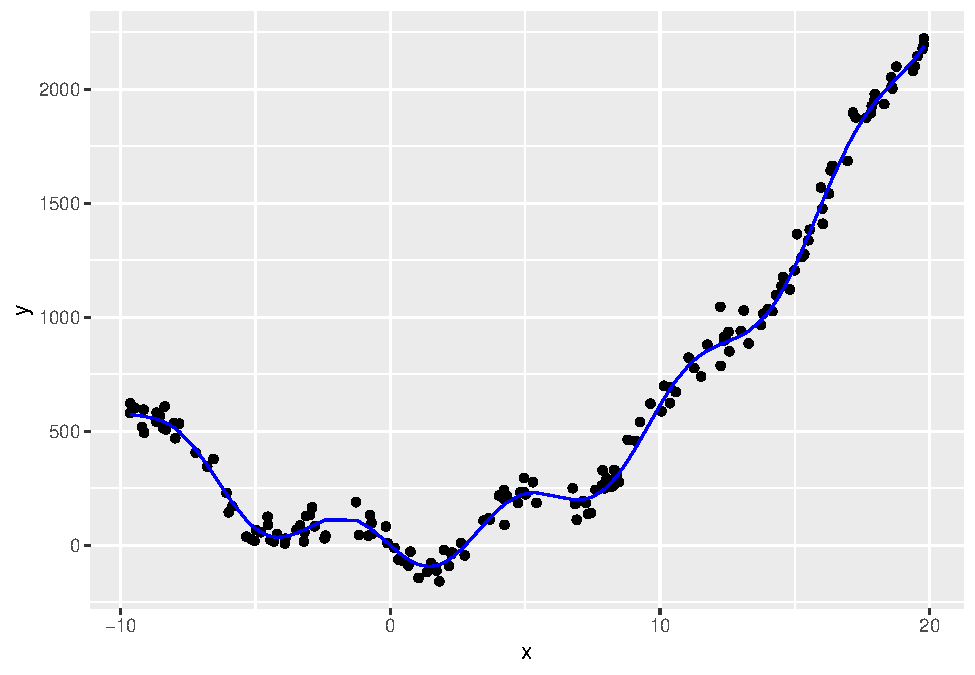
\includegraphics{assignment1_files/figure-latex/unnamed-chunk-2-1.pdf}

\begin{enumerate}
\def\labelenumi{\alph{enumi}.}
\setcounter{enumi}{1}
\tightlist
\item
  (1)Break the data into a \(2/3\) training and a \(1/3\) test set.
  (Hint: You can use the function \texttt{createDataPartition} from the
  \texttt{caret} package.) Fit a linear model, using the training set.
  Compute the training MSE and test MSE. Overlay the linear model fit on
  a plot of the data and true model.
\end{enumerate}

\begin{Shaded}
\begin{Highlighting}[]
\CommentTok{# Create training and test sets}
\KeywordTok{set.seed}\NormalTok{(}\DecValTok{20200318}\NormalTok{)}
\NormalTok{tr_indx <-}\StringTok{ }\KeywordTok{createDataPartition}\NormalTok{(df}\OperatorTok{$}\NormalTok{y, }\DataTypeTok{p=}\FloatTok{0.66}\NormalTok{)}\OperatorTok{$}\NormalTok{Resample1}
\NormalTok{tr <-}\StringTok{ }\NormalTok{df[tr_indx,]}
\NormalTok{ts <-}\StringTok{ }\NormalTok{df[}\OperatorTok{-}\NormalTok{tr_indx,]}

\CommentTok{# Fit linear model}
\NormalTok{fit1 <-}\StringTok{ }\KeywordTok{lm}\NormalTok{(y}\OperatorTok{~}\NormalTok{x, }\DataTypeTok{data=}\NormalTok{tr)}
\NormalTok{tr_aug <-}\StringTok{ }\KeywordTok{augment}\NormalTok{(fit1, tr)}
\NormalTok{ts_aug <-}\StringTok{ }\KeywordTok{augment}\NormalTok{(fit1, }\DataTypeTok{newdata=}\NormalTok{ts)}
\NormalTok{ts_aug}\OperatorTok{$}\NormalTok{.resid <-}\StringTok{ }\NormalTok{ts_aug}\OperatorTok{$}\NormalTok{y }\OperatorTok{-}\StringTok{ }\NormalTok{ts_aug}\OperatorTok{$}\NormalTok{.fitted}
\NormalTok{tr_mse <-}\StringTok{ }\KeywordTok{sum}\NormalTok{((tr_aug}\OperatorTok{$}\NormalTok{y}\OperatorTok{-}\NormalTok{tr_aug}\OperatorTok{$}\NormalTok{.fitted)}\OperatorTok{^}\DecValTok{2}\NormalTok{)}\OperatorTok{/}\KeywordTok{length}\NormalTok{(ts_aug}\OperatorTok{$}\NormalTok{.fitted)}
\NormalTok{ts_mse <-}\StringTok{ }\KeywordTok{sum}\NormalTok{(ts_aug}\OperatorTok{$}\NormalTok{.resid}\OperatorTok{^}\DecValTok{2}\NormalTok{)}\OperatorTok{/}\KeywordTok{length}\NormalTok{(ts_aug}\OperatorTok{$}\NormalTok{.resid)}

\KeywordTok{print}\NormalTok{(}\KeywordTok{c}\NormalTok{(}\StringTok{'Training MSE:'}\NormalTok{,tr_mse,}\StringTok{'Test MSE:'}\NormalTok{, ts_mse))}
\end{Highlighting}
\end{Shaded}

\begin{verbatim}
## [1] "Training MSE:"    "355934.382193997" "Test MSE:"        "223652.69872877"
\end{verbatim}

\begin{Shaded}
\begin{Highlighting}[]
\CommentTok{# Plot the data, true model and fitted model}
\KeywordTok{ggplot}\NormalTok{(df, }\KeywordTok{aes}\NormalTok{(}\DataTypeTok{x=}\NormalTok{x, }\DataTypeTok{y=}\NormalTok{y)) }\OperatorTok{+}\StringTok{ }\KeywordTok{geom_point}\NormalTok{() }\OperatorTok{+}
\StringTok{  }\KeywordTok{geom_line}\NormalTok{(}\KeywordTok{aes}\NormalTok{(}\DataTypeTok{y=}\NormalTok{true)) }\OperatorTok{+}\StringTok{ }\KeywordTok{geom_point}\NormalTok{(}\DataTypeTok{data=}\NormalTok{fit1, }\KeywordTok{aes}\NormalTok{(}\DataTypeTok{x=}\NormalTok{x, }\DataTypeTok{y=}\NormalTok{.fitted), }\DataTypeTok{colour=}\StringTok{"orange"}\NormalTok{)}
\end{Highlighting}
\end{Shaded}

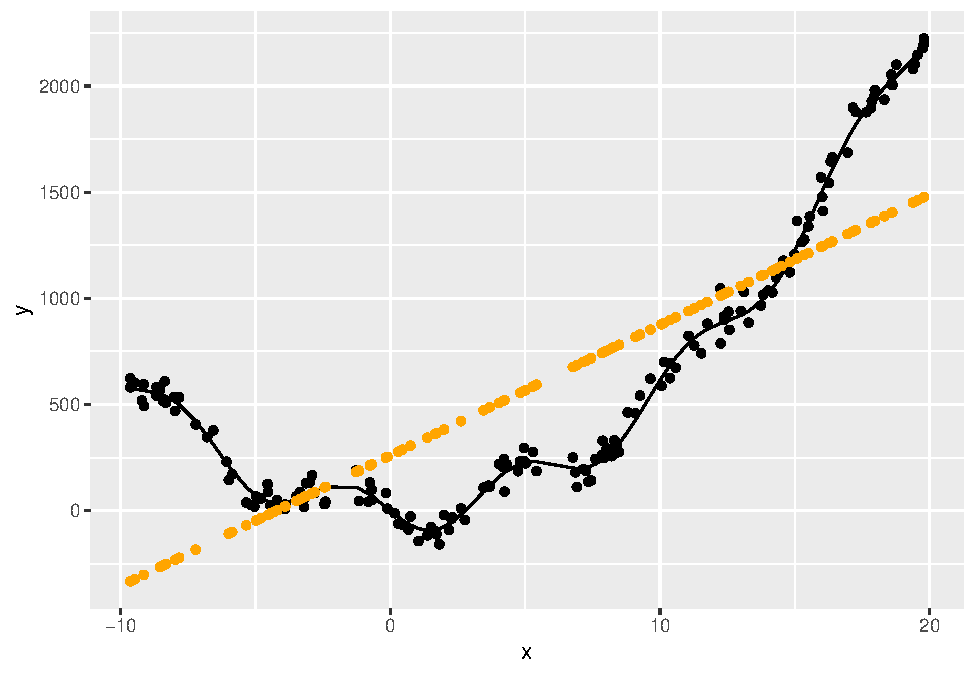
\includegraphics{assignment1_files/figure-latex/unnamed-chunk-3-1.pdf}

\begin{enumerate}
\def\labelenumi{\alph{enumi}.}
\setcounter{enumi}{2}
\tightlist
\item
  Now examine the behaviour of the training and test MSE, for a
  \texttt{loess} fit.

  \begin{enumerate}
  \def\labelenumii{\roman{enumii}.}
  \tightlist
  \item
    (1)Look up the \texttt{loess} model fit, and write a paragraph
    explaining how this fitting procedure works. In particular, explain
    what the \texttt{span} argument does. Add a (hand) sketch
    illustrating the method.
  \end{enumerate}
\end{enumerate}

Loess stands for local regression, and it works by binning your
observations into categories based on a dependant variable, this means
that different regions can have different relationships. The span
argument controls how small the bins are, the smaller they are the more
flexible the data is in that it can model more complex relationships.
The larger the span/bins are the smoother the fitted data is.

\begin{figure}
\centering
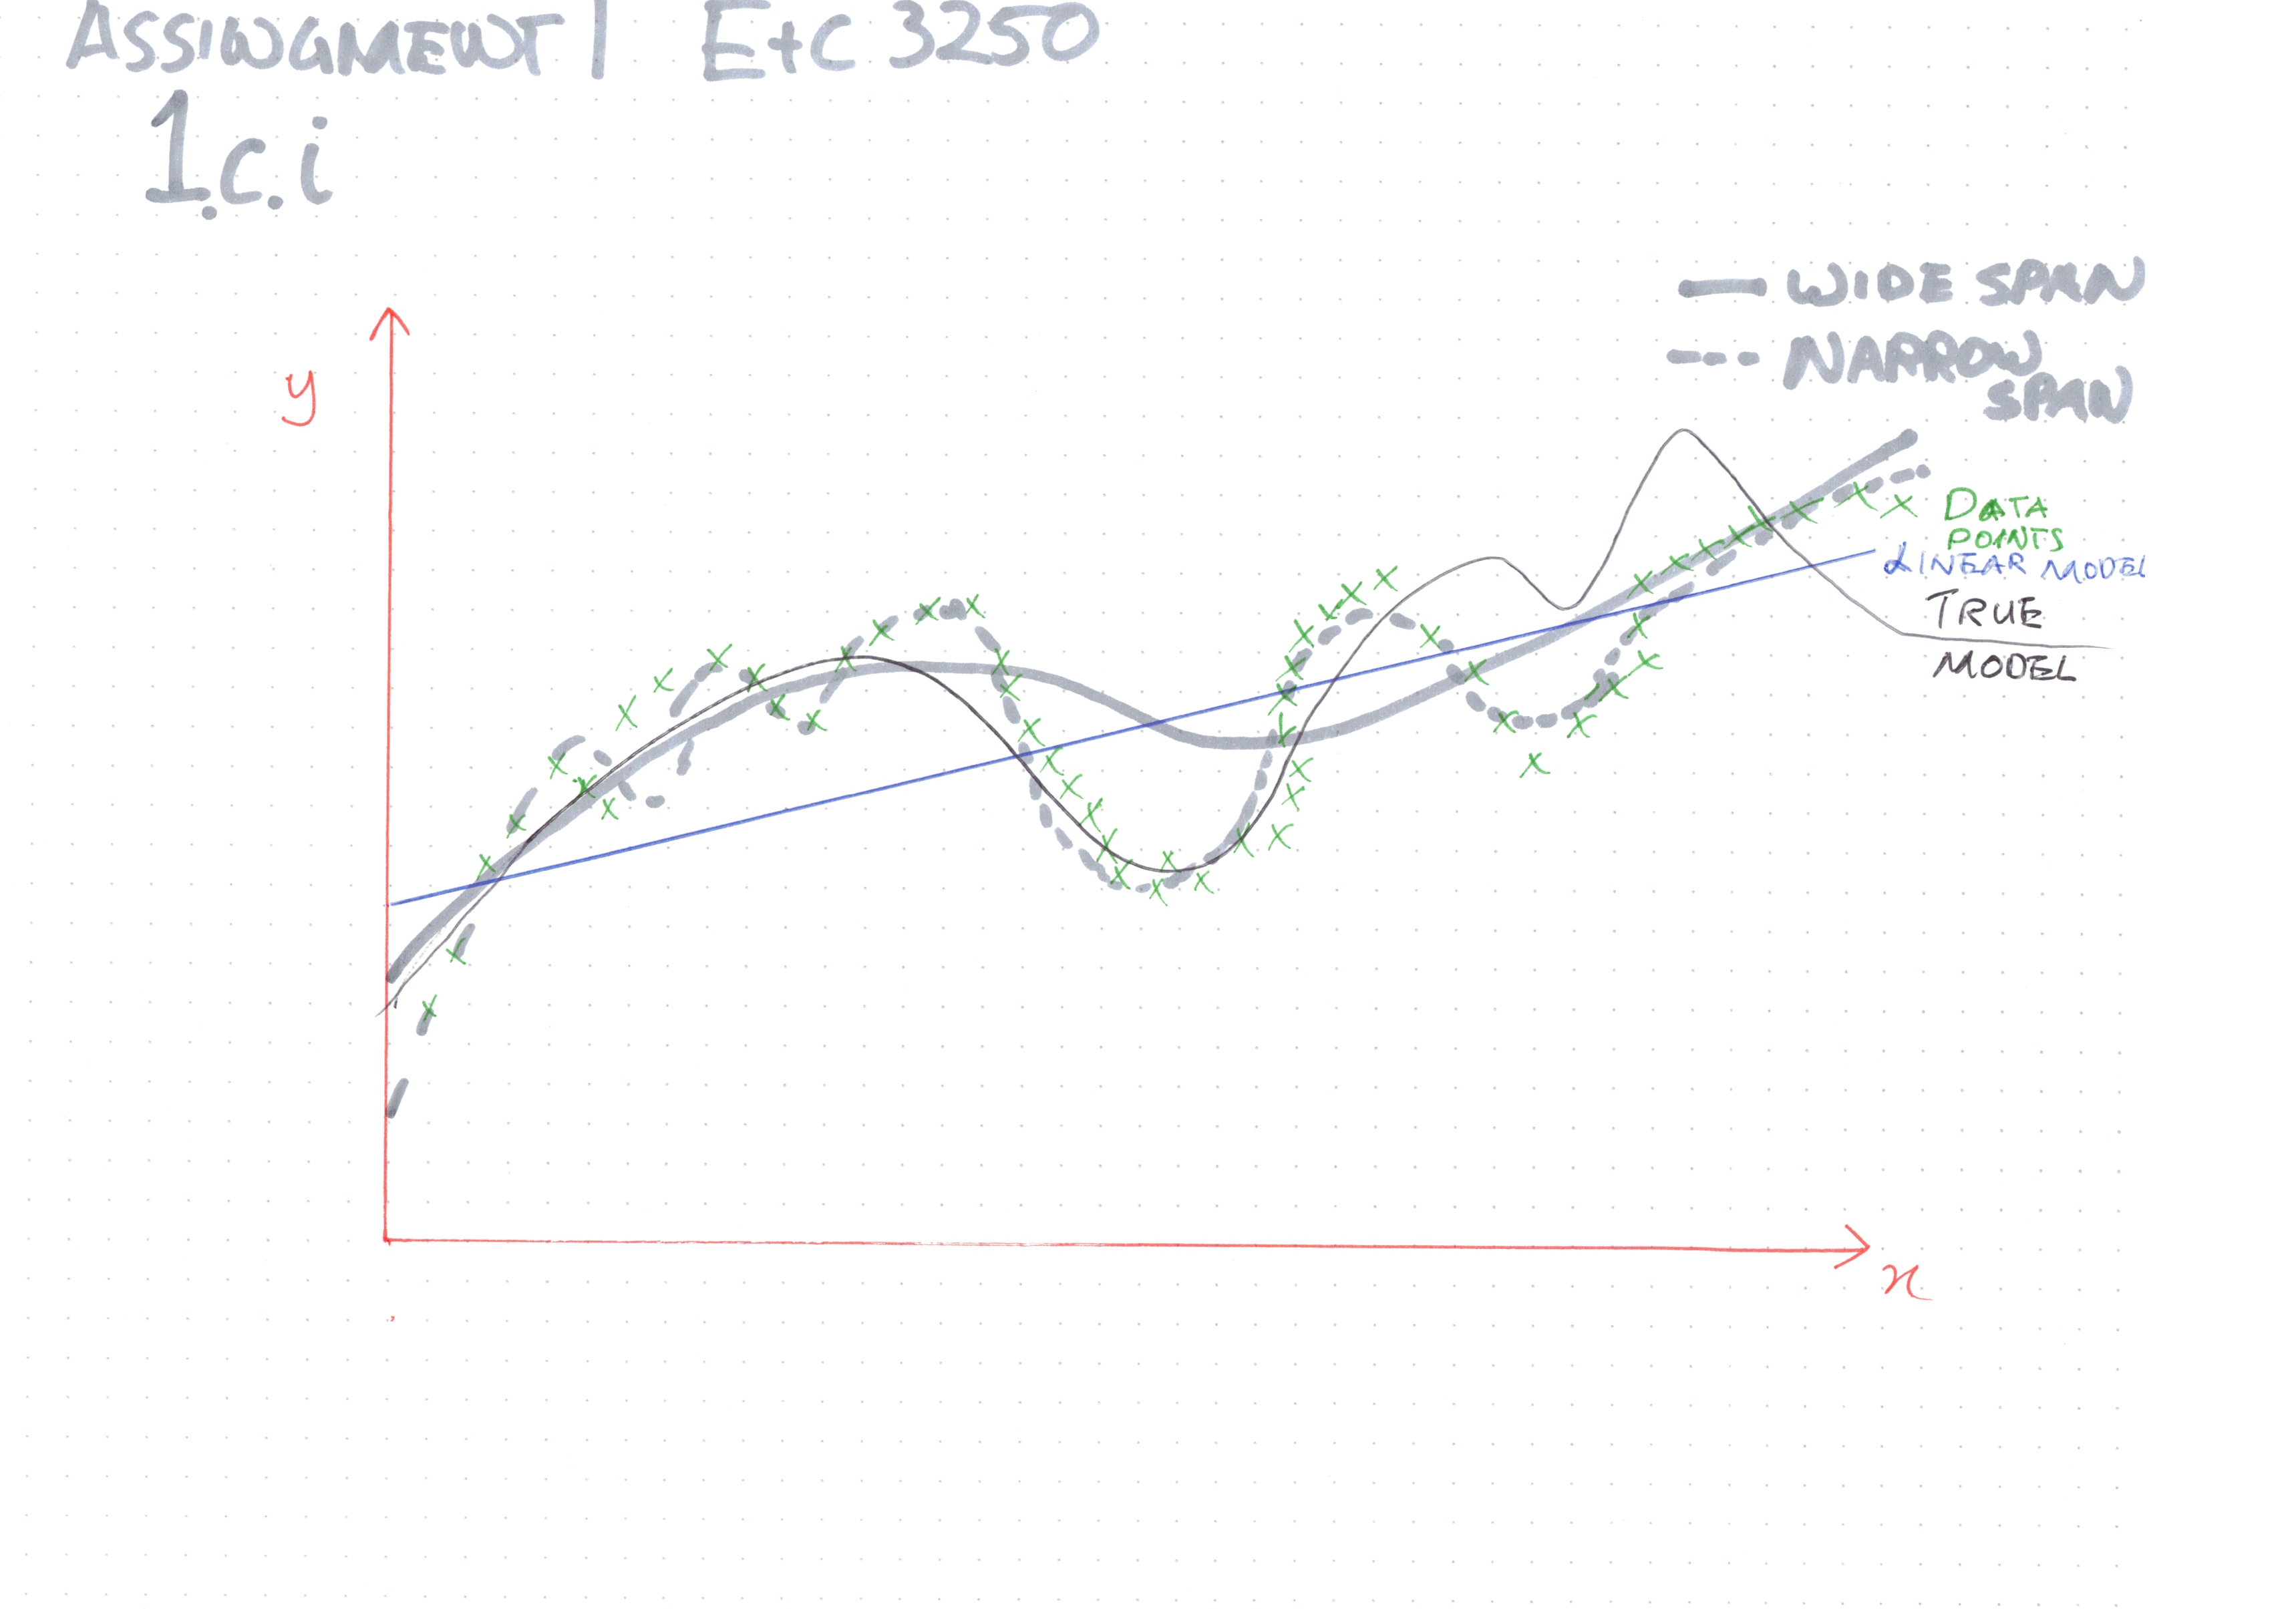
\includegraphics{https://raw.githubusercontent.com/jlgao2/ETC3250/master/images/CCI_000002.png}
\caption{here is the sketch}
\end{figure}

\begin{verbatim}
ii. (1)Compute the training and test MSE for a range of `span` values, 2, 1, 0.5, 0.3, 0.2, 0.1, 0.05. Plot the training and test MSE against the span parameter. For each model, also make a plot of the data and fitted model. Include just the plot of the fit of the model that you think best captures the relationship between x and y.)
\end{verbatim}

\begin{Shaded}
\begin{Highlighting}[]
\NormalTok{span <-}\StringTok{ }\KeywordTok{c}\NormalTok{(}\DecValTok{2}\NormalTok{, }\DecValTok{1}\NormalTok{, }\FloatTok{0.5}\NormalTok{, }\FloatTok{0.3}\NormalTok{, }\FloatTok{0.2}\NormalTok{, }\FloatTok{0.1}\NormalTok{, }\FloatTok{0.05}\NormalTok{)}
\NormalTok{tr_mse2 <-}\StringTok{ }\OtherTok{NULL}
\NormalTok{ts_mse2 <-}\StringTok{ }\OtherTok{NULL}

\CommentTok{# Fit a loess model and compute MSEs}
\ControlFlowTok{for}\NormalTok{ (i }\ControlFlowTok{in} \DecValTok{1}\OperatorTok{:}\KeywordTok{length}\NormalTok{(span)) }
\NormalTok{  \{}
\NormalTok{  fit2 <-}\StringTok{ }\KeywordTok{loess}\NormalTok{(y}\OperatorTok{~}\NormalTok{x, }\DataTypeTok{data=}\NormalTok{tr, }\DataTypeTok{span=}\NormalTok{span[i])}
\NormalTok{  tr_aug2 <-}\StringTok{ }\KeywordTok{augment}\NormalTok{(fit2, tr)}
\NormalTok{  ts_aug2 <-}\StringTok{ }\KeywordTok{augment}\NormalTok{(fit2, }\DataTypeTok{newdata=}\NormalTok{ts)}
\NormalTok{  ts_aug2}\OperatorTok{$}\NormalTok{.resid <-}\StringTok{ }\NormalTok{ts_aug2}\OperatorTok{$}\NormalTok{y }\OperatorTok{-}\StringTok{ }\NormalTok{ts_aug2}\OperatorTok{$}\NormalTok{.fitted}
\NormalTok{  trm <-}\StringTok{ }\KeywordTok{sum}\NormalTok{((tr_aug2}\OperatorTok{$}\NormalTok{y}\OperatorTok{-}\NormalTok{tr_aug2}\OperatorTok{$}\NormalTok{.fitted)}\OperatorTok{^}\DecValTok{2}\NormalTok{)}\OperatorTok{/}\KeywordTok{length}\NormalTok{(tr_aug2)}
\NormalTok{  tsm <-}\StringTok{ }\KeywordTok{sum}\NormalTok{(ts_aug2}\OperatorTok{$}\NormalTok{.resid}\OperatorTok{^}\DecValTok{2}\NormalTok{, }\DataTypeTok{na.rm=}\OtherTok{TRUE}\NormalTok{)}\OperatorTok{/}
\StringTok{    }\KeywordTok{length}\NormalTok{(tr_aug2)}
\NormalTok{  tr_mse2 <-}\StringTok{ }\KeywordTok{c}\NormalTok{(tr_mse2, trm)}
\NormalTok{  ts_mse2 <-}\StringTok{ }\KeywordTok{c}\NormalTok{(ts_mse2, tsm)}
\NormalTok{\}}

\NormalTok{mse_df <-}\StringTok{ }\KeywordTok{tibble}\NormalTok{(span, }\StringTok{`}\DataTypeTok{train MSE}\StringTok{`}\NormalTok{=tr_mse2, }\StringTok{`}\DataTypeTok{test MSE}\StringTok{`}\NormalTok{=ts_mse2)}
\NormalTok{mse_df <-}\StringTok{ }\NormalTok{mse_df }\OperatorTok\StringTok{ }
\StringTok{  }\KeywordTok{pivot_longer}\NormalTok{(}\DataTypeTok{cols =} \OperatorTok{-}\NormalTok{span, }\DataTypeTok{names_to =} \StringTok{"type"}\NormalTok{, }\DataTypeTok{values_to=}\StringTok{"mse"}\NormalTok{)}
\KeywordTok{ggplot}\NormalTok{(mse_df, }\KeywordTok{aes}\NormalTok{(}\DataTypeTok{x=}\NormalTok{span, }\DataTypeTok{y=}\NormalTok{mse, }\DataTypeTok{colour=}\NormalTok{type)) }\OperatorTok{+}\StringTok{ }
\StringTok{  }\KeywordTok{geom_col}\NormalTok{(}\DataTypeTok{position=}\StringTok{"dodge"}\NormalTok{) }\OperatorTok{+}
\StringTok{  }\KeywordTok{geom_line}\NormalTok{() }\OperatorTok{+}
\StringTok{  }\KeywordTok{scale_x_reverse}\NormalTok{() }\OperatorTok{+}
\StringTok{  }\KeywordTok{ylab}\NormalTok{(}\StringTok{"MSE"}\NormalTok{) }\OperatorTok{+}
\StringTok{  }\KeywordTok{scale_colour_brewer}\NormalTok{(}\StringTok{""}\NormalTok{, }\DataTypeTok{palette=}\StringTok{"Dark2"}\NormalTok{)}
\end{Highlighting}
\end{Shaded}

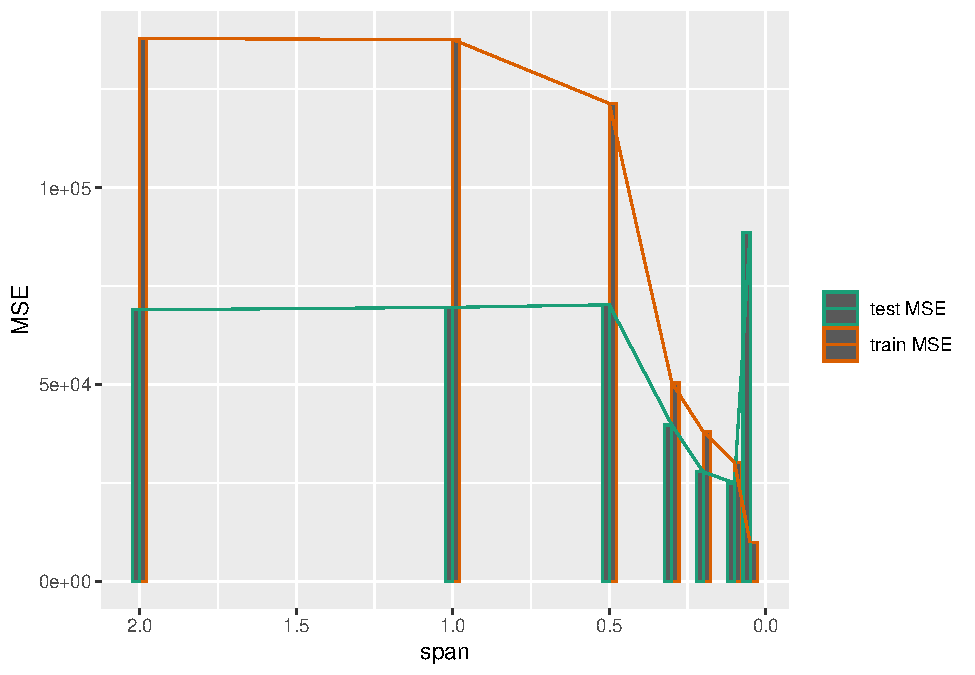
\includegraphics{assignment1_files/figure-latex/unnamed-chunk-4-1.pdf}

\begin{verbatim}
iii. (2)Write a paragraph explaining the effect of increasing the flexibility of the fit has on the training and test MSE. Indicate what you think is the optimal span value for this data. Make a plot of this optimal fit.
\end{verbatim}

\begin{Shaded}
\begin{Highlighting}[]
\NormalTok{fit_all <-}\StringTok{ }\KeywordTok{loess}\NormalTok{(y}\OperatorTok{~}\NormalTok{x, }\DataTypeTok{data=}\NormalTok{df, }\DataTypeTok{span=}\FloatTok{0.1}\NormalTok{)}
\NormalTok{df_all <-}\StringTok{ }\KeywordTok{augment}\NormalTok{(fit_all)}
\KeywordTok{ggplot}\NormalTok{(df, }\KeywordTok{aes}\NormalTok{(}\DataTypeTok{x=}\NormalTok{x, }\DataTypeTok{y=}\NormalTok{y)) }\OperatorTok{+}\StringTok{ }\KeywordTok{geom_point}\NormalTok{() }\OperatorTok{+}
\StringTok{  }\KeywordTok{geom_line}\NormalTok{(}\DataTypeTok{data=}\NormalTok{df_all, }\KeywordTok{aes}\NormalTok{(x, }\DataTypeTok{y=}\NormalTok{.fitted), }\DataTypeTok{size =} \DecValTok{2}\NormalTok{, }\DataTypeTok{colour=}\StringTok{"orange"}\NormalTok{)}
\end{Highlighting}
\end{Shaded}

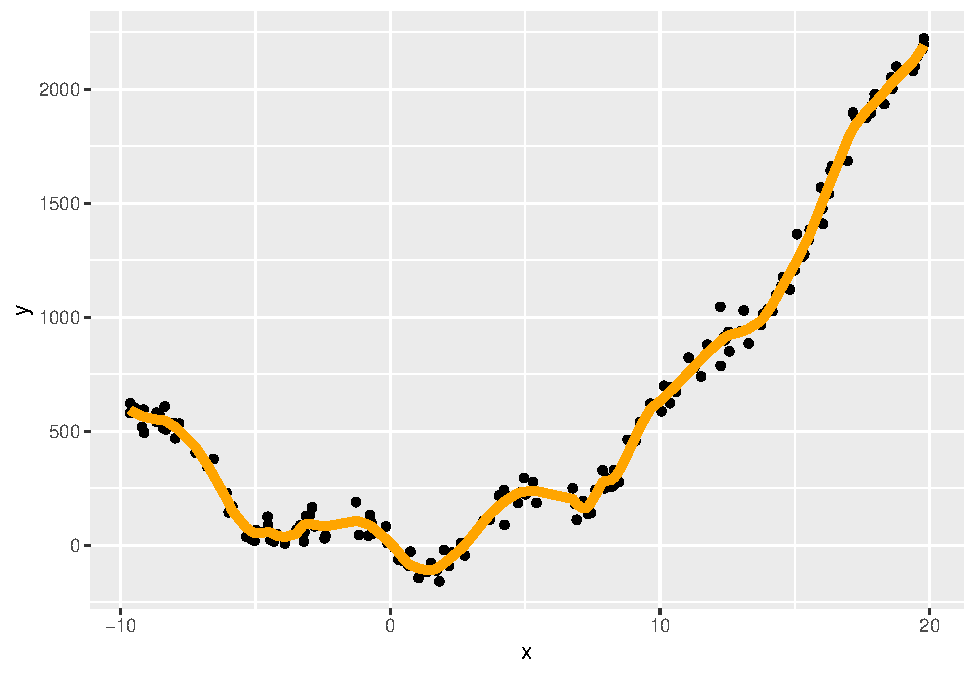
\includegraphics{assignment1_files/figure-latex/unnamed-chunk-5-1.pdf}

\begin{enumerate}
\def\labelenumi{\alph{enumi}.}
\setcounter{enumi}{3}
\tightlist
\item
  (2)Make a sketch indicating observed data, the true model, fitted
  model, and indicate what the bias, variance and MSE refer to. Remember
  that to understand bias and variance, you need to think about taking
  multiple (and actually all possible) samples. Your illustration would
  have predictor (\(x\)) on the horizontal axis and response on the
  vertical axis. Represent and observed value with a dot, and use curves
  for fitted models and the true model.
\end{enumerate}

\begin{figure}
\centering
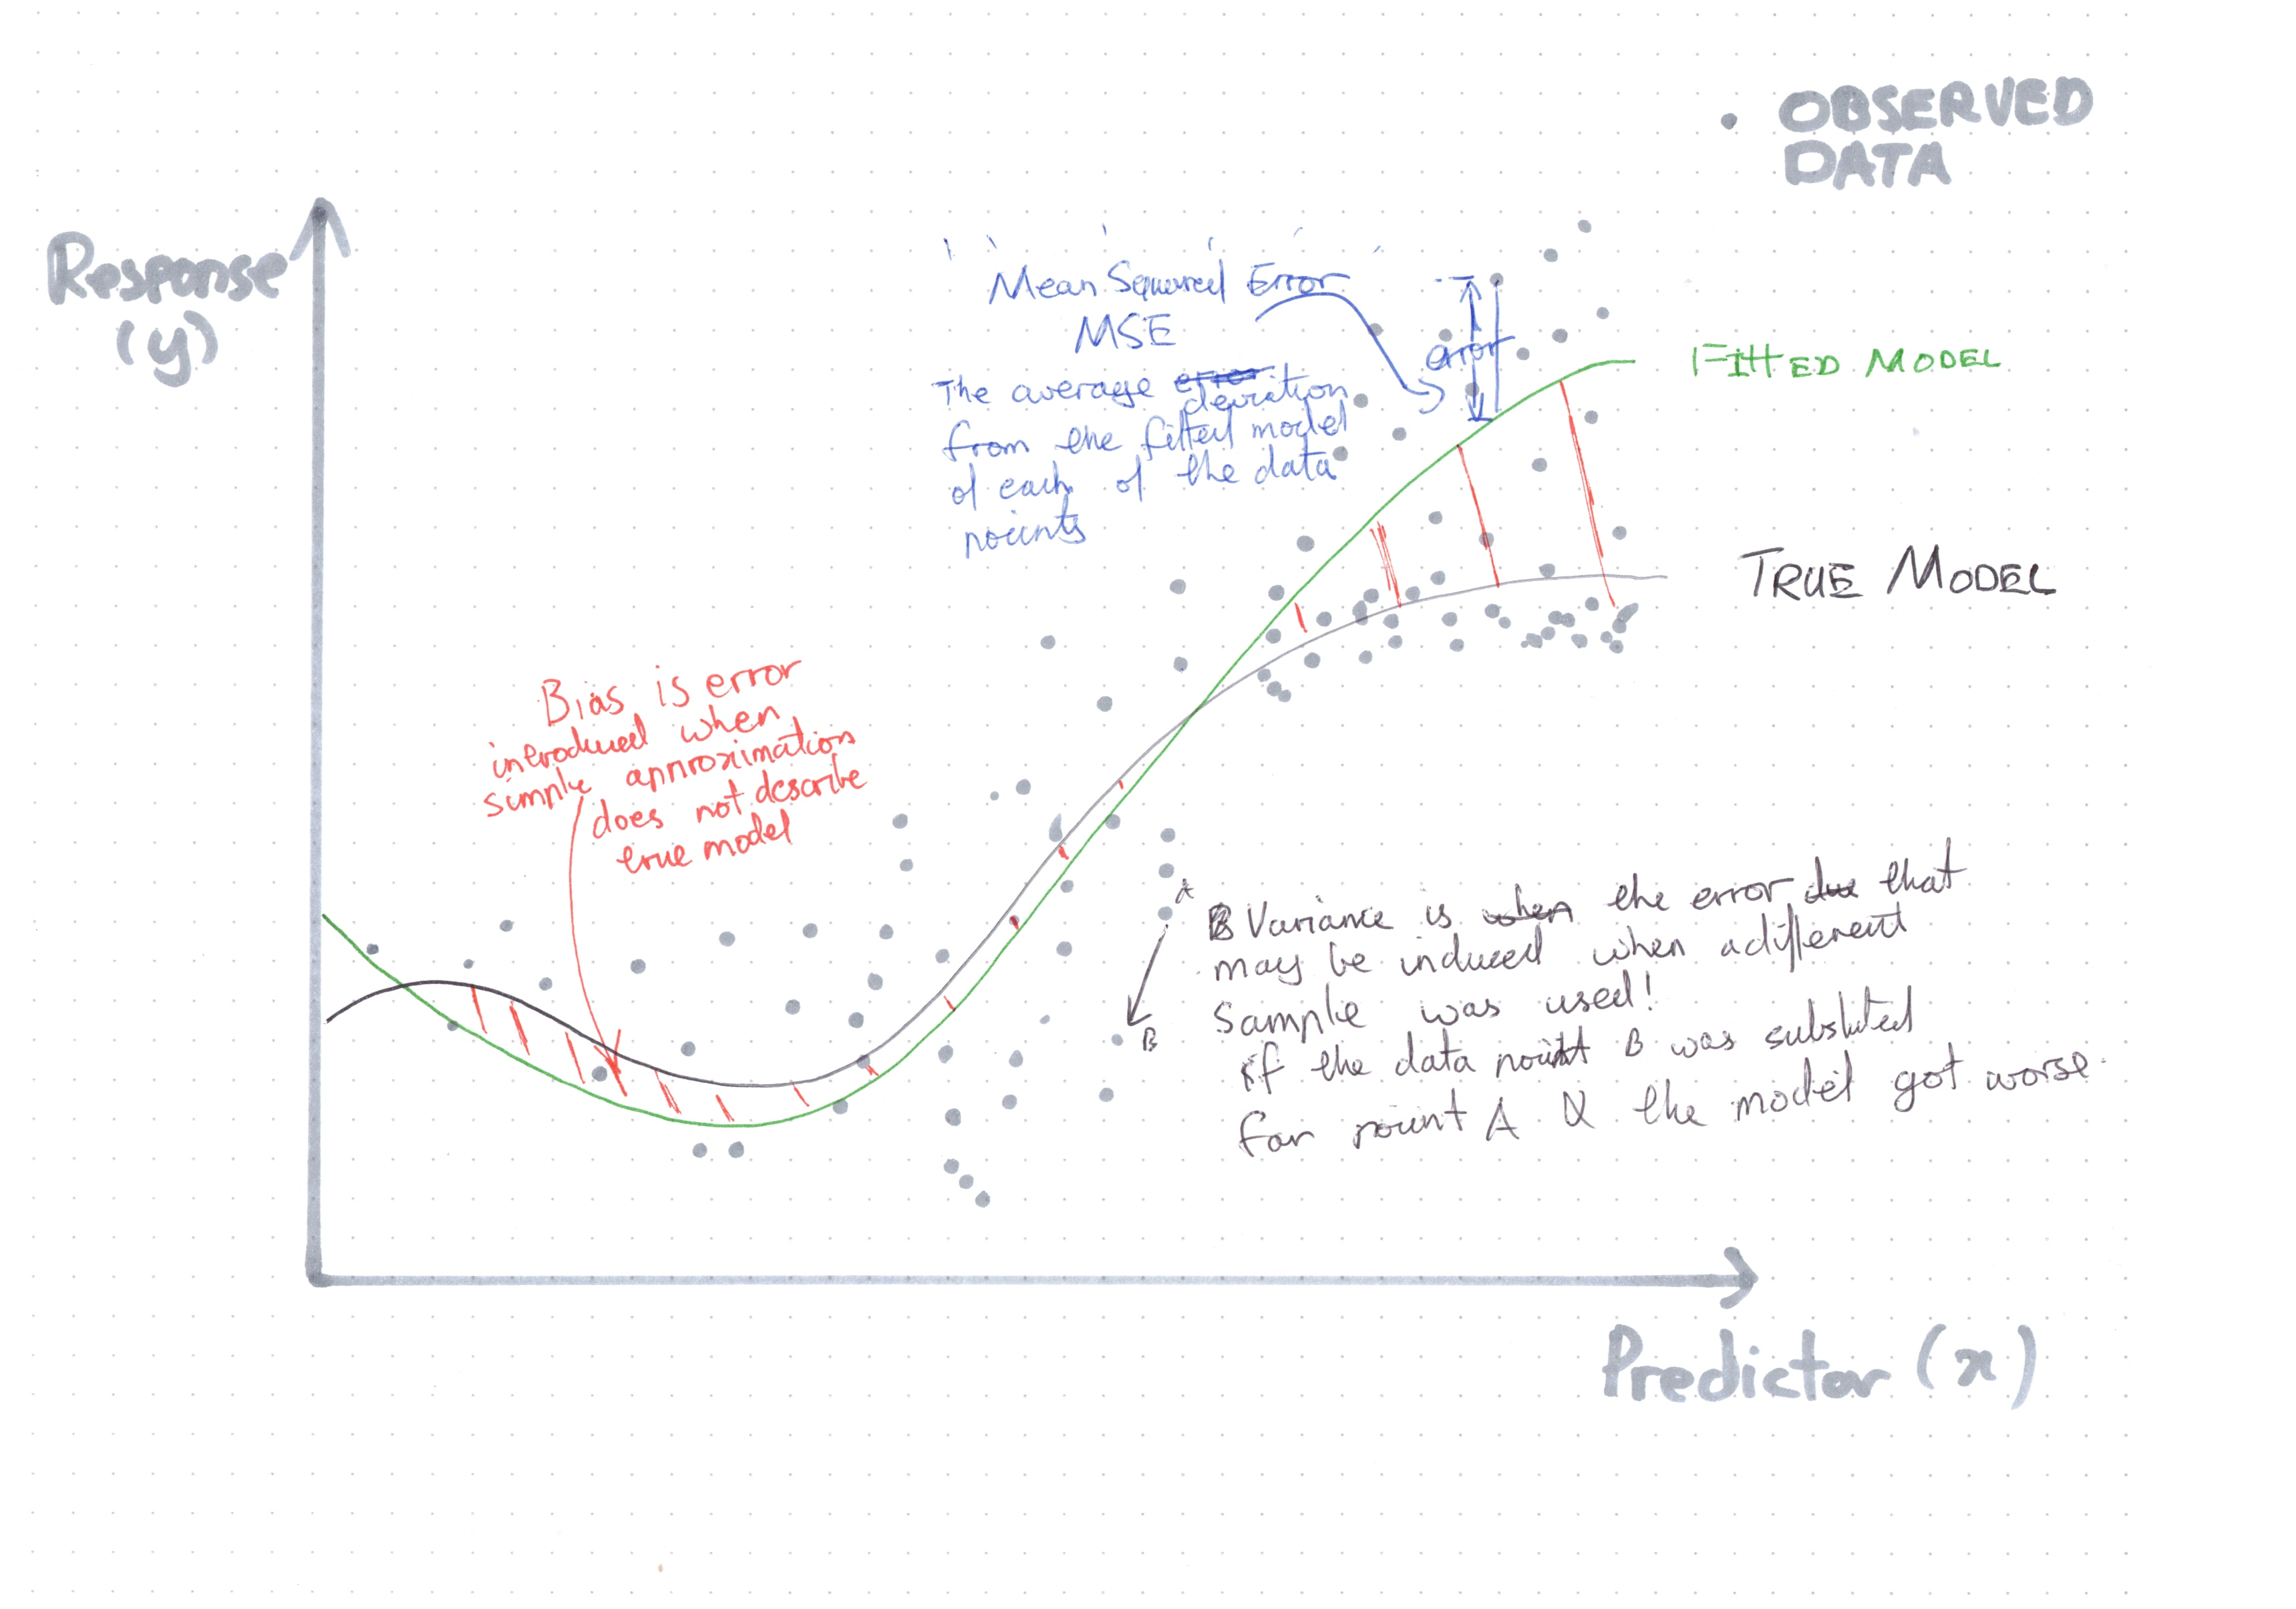
\includegraphics{https://raw.githubusercontent.com/jlgao2/ETC3250/master/images/CCI_000001.png}
\caption{here is another}
\end{figure}

\begin{enumerate}
\def\labelenumi{\arabic{enumi}.}
\setcounter{enumi}{1}
\tightlist
\item
  The current COVID-19 health crisis worries us all. John Hopkins
  University has been carefully documenting incidence, recoveries and
  deaths around the globe. Read the incidence data from
  \url{https://raw.githubusercontent.com/CSSEGISandData/COVID-19/master/csse_covid_19_data/csse_covid_19_time_series/time_series_19-covid-Confirmed.csv},
  into R.
\end{enumerate}

\begin{enumerate}
\def\labelenumi{\alph{enumi}.}
\tightlist
\item
  (2)The data shows cumulative counts by date for many countries.
  Extract the data for Australia. It is currently multiple rows
  corresponding to counts in different states. Pivot the data into long
  tidy form, and convert the text date into a date variable. Difference
  the days, so that you have the incidence for each day. Make a bar
  chart of incidence by date. Add a loess smooth to the plot.
\end{enumerate}

\begin{Shaded}
\begin{Highlighting}[]
\KeywordTok{library}\NormalTok{(lubridate)}
\KeywordTok{library}\NormalTok{(tsibble)}
\NormalTok{covid_jh <-}\StringTok{ }\KeywordTok{read_csv}\NormalTok{(}\StringTok{"https://raw.githubusercontent.com/CSSEGISandData/COVID-19/master/csse_covid_19_data/csse_covid_19_time_series/time_series_covid19_confirmed_global.csv"}\NormalTok{)}
\NormalTok{covid_jh_oz <-}\StringTok{ }\NormalTok{covid_jh }\OperatorTok
\StringTok{  }\KeywordTok{filter}\NormalTok{(}\StringTok{`}\DataTypeTok{Country/Region}\StringTok{`} \OperatorTok{==}\StringTok{ "Australia"}\NormalTok{) }\OperatorTok
\StringTok{  }\KeywordTok{pivot_longer}\NormalTok{(}\DataTypeTok{cols =} \KeywordTok{ends_with}\NormalTok{(}\StringTok{"20"}\NormalTok{), }\DataTypeTok{names_to =} \StringTok{"date"}\NormalTok{) }\OperatorTok
\StringTok{  }\KeywordTok{mutate}\NormalTok{(}\DataTypeTok{date =} \KeywordTok{mdy}\NormalTok{(date)) }\OperatorTok
\StringTok{  }\KeywordTok{group_by}\NormalTok{(date) }\OperatorTok
\StringTok{  }\KeywordTok{summarise}\NormalTok{(}\DataTypeTok{count =} \KeywordTok{sum}\NormalTok{(value)) }\OperatorTok
\StringTok{  }\KeywordTok{mutate}\NormalTok{(}\DataTypeTok{dif =} \KeywordTok{c}\NormalTok{(}\OtherTok{NA}\NormalTok{, }\KeywordTok{diff}\NormalTok{(count)))}
\NormalTok{covid_jh_oz }\OperatorTok
\StringTok{  }\KeywordTok{ggplot}\NormalTok{(}\KeywordTok{aes}\NormalTok{(}\DataTypeTok{x=}\NormalTok{date, }\DataTypeTok{y=}\NormalTok{dif)) }\OperatorTok{+}\StringTok{ }
\StringTok{  }\KeywordTok{geom_col}\NormalTok{() }\OperatorTok{+}
\StringTok{  }\KeywordTok{geom_smooth}\NormalTok{(}\DataTypeTok{se=}\OtherTok{FALSE}\NormalTok{) }\OperatorTok{+}
\StringTok{  }\KeywordTok{ylab}\NormalTok{(}\StringTok{"New Cases Incidence"}\NormalTok{) }\OperatorTok{+}\StringTok{ }\KeywordTok{xlab}\NormalTok{(}\StringTok{"date"}\NormalTok{)}
\end{Highlighting}
\end{Shaded}

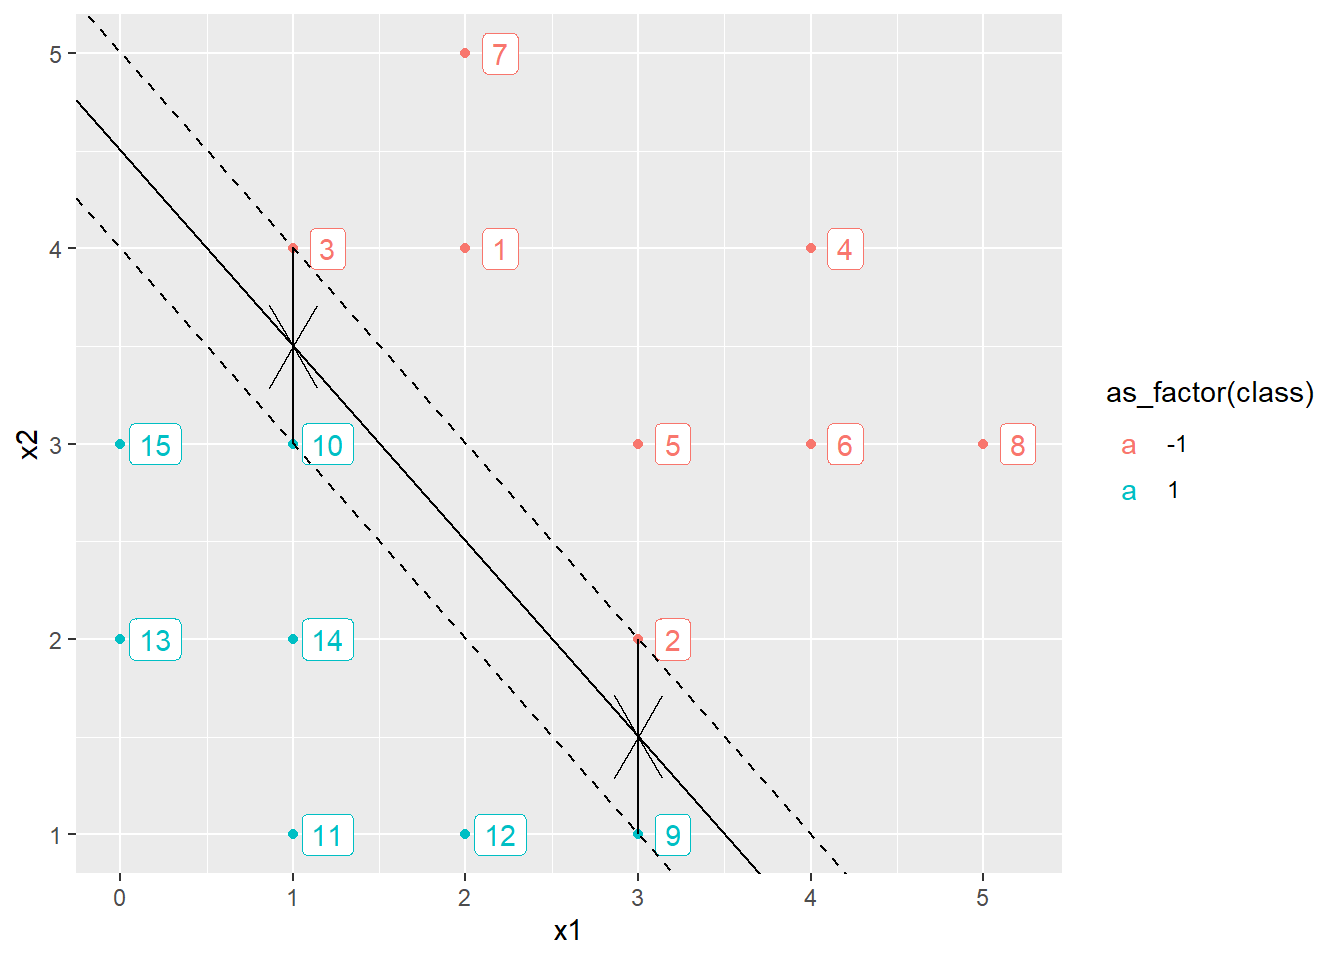
\includegraphics{assignment1_files/figure-latex/unnamed-chunk-6-1.pdf}

\begin{enumerate}
\def\labelenumi{\alph{enumi}.}
\setcounter{enumi}{1}
\tightlist
\item
  (3)Fit an appropriate linear model, using \texttt{glm} to the data.
  (Hint: ) Make a summary of the model fit, write down the model
  equation and a plot of the data with the model overlaid. Compute the
  ratio of the deviance relative to the null deviance. What does this
  say about the model fit? Is it a good summary of the variation in
  counts?
\end{enumerate}

\begin{Shaded}
\begin{Highlighting}[]
\NormalTok{covid_jh_oz_lm <-}\StringTok{ }\KeywordTok{glm}\NormalTok{(dif}\OperatorTok{~}\NormalTok{date, }\DataTypeTok{data=}\NormalTok{covid_jh_oz, }\DataTypeTok{family=}\NormalTok{gaussian)}
\NormalTok{covid_jh_oz_lm}
\end{Highlighting}
\end{Shaded}

\begin{verbatim}
## 
## Call:  glm(formula = dif ~ date, family = gaussian, data = covid_jh_oz)
## 
## Coefficients:
## (Intercept)         date  
##   -75417.78         4.12  
## 
## Degrees of Freedom: 65 Total (i.e. Null);  64 Residual
##   (1 observation deleted due to missingness)
## Null Deviance:       975900 
## Residual Deviance: 569200    AIC: 791.4
\end{verbatim}

\begin{Shaded}
\begin{Highlighting}[]
\NormalTok{covid_jh_oz <-}\StringTok{  }\KeywordTok{augment}\NormalTok{(covid_jh_oz_lm) }\CommentTok{#%>%}
\CommentTok{#  mutate(.fitted =)}
\NormalTok{covid_jh_oz }\OperatorTok
\StringTok{  }\KeywordTok{ggplot}\NormalTok{(}\KeywordTok{aes}\NormalTok{(}\DataTypeTok{x=}\NormalTok{date, }\DataTypeTok{y=}\NormalTok{dif)) }\OperatorTok{+}
\StringTok{  }\KeywordTok{geom_col}\NormalTok{() }\OperatorTok{+}
\StringTok{  }\KeywordTok{geom_smooth}\NormalTok{(}\DataTypeTok{se=}\OtherTok{FALSE}\NormalTok{) }\OperatorTok{+}
\StringTok{  }\KeywordTok{geom_line}\NormalTok{(}\KeywordTok{aes}\NormalTok{(}\DataTypeTok{y=}\NormalTok{.fitted), }\DataTypeTok{color=}\StringTok{"red"}\NormalTok{) }\OperatorTok{+}
\StringTok{  }\KeywordTok{xlab}\NormalTok{(}\StringTok{"date"}\NormalTok{) }\OperatorTok{+}\StringTok{ }\KeywordTok{ylab}\NormalTok{(}\StringTok{"daily count"}\NormalTok{) }
\end{Highlighting}
\end{Shaded}

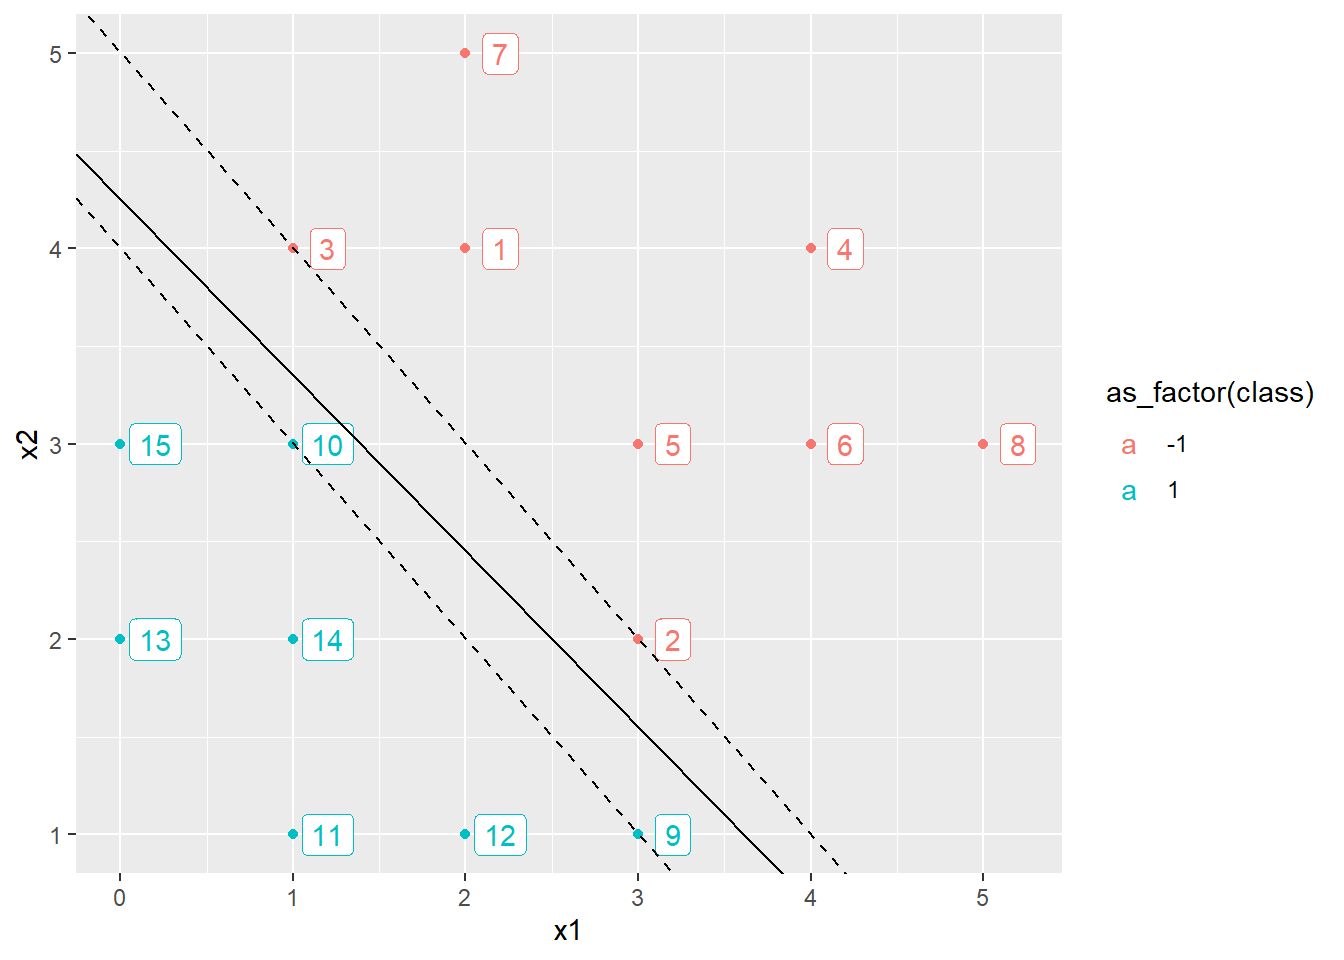
\includegraphics{assignment1_files/figure-latex/unnamed-chunk-7-1.pdf}

\begin{enumerate}
\def\labelenumi{\alph{enumi}.}
\setcounter{enumi}{3}
\tightlist
\item
  (1)Would the \texttt{glm} model be considered a flexible or inflexible
  model? Inflexible
\item
  (1)Use your model to predict the count for Mar 31.
\end{enumerate}

\begin{Shaded}
\begin{Highlighting}[]
\KeywordTok{predict}\NormalTok{(covid_jh_oz_lm, }\DataTypeTok{newdata=}\KeywordTok{data.frame}\NormalTok{(}\DataTypeTok{date =} \KeywordTok{dmy}\NormalTok{(}\StringTok{"31/3/20"}\NormalTok{)))}
\end{Highlighting}
\end{Shaded}

\begin{verbatim}
##        1 
## 201.4289
\end{verbatim}

There will be

\end{document}
